% =============================== 7. Q4 ===============================
\section{Question 4: Siting and Sizing Electronic Fences}\label{sec:q4}

\subsection{Parking demand is the arrival process}

A dockless bicycle occupies space where its trip ends, and it stays there until someone
rides it away. The demand for parking at a cell is therefore the arrival process ---
which the model of Section~\ref{sec:q1} predicts --- and the capacity of a fence is
the number of bicycles that can be standing inside it at the worst moment of the day.

Capacity is sized by Monte Carlo. For a candidate fence serving a set $S$ of cells we
draw Poisson arrivals and departures on the 15-minute grid,
\begin{equation}
o_{t+1} \;=\; \max\left\{0,\ o_t + A_t - D_t\right\},
\qquad A_t\sim\text{Poisson}\!\left(\textstyle\sum_{c\in S}a_{ct}\right),
\quad D_t\sim\text{Poisson}\!\left(\textstyle\sum_{c\in S}d_{ct}\right),
\end{equation}
record the peak $\max_t o_t$ over 96 intervals, repeat 300 times, and set the capacity
to the 95th percentile of the simulated peaks. Two conventions are worth stating. The
occupancy starts at zero, which is consistent with the nightly reset of
Section~\ref{sec:q2}: fences are emptied overnight and refilled by the day's arrivals.
And the arrival rate is the scaled one, $1/p$ times the sample, so the capacities are
those of the real system rather than of the sample.

\subsection{Where to put the fences}

Siting is a maximal-coverage problem. A fence at cell $c$ with walking radius $R$
serves every arrival whose destination lies within $R$ of $c$; the planner chooses a
set of fences to cover as many arrivals as possible. The problem is NP-hard but its
objective is submodular, so the greedy algorithm --- repeatedly place the fence that
covers the most still-uncovered arrivals --- attains at least $(1-1/e)=63.2\%$ of the
optimum \cite{nemhauser1978}. With 5{,}263 cells and 2{,}500 candidate sites the greedy
pass runs in seconds and the bound is comfortable.

\begin{table}[htbp]
\centering
\caption[Fence plans]{Fence plans. Coverage is the share of daily arrivals inside some fence's
walking radius; capacity is the Monte-Carlo 95th-percentile peak occupancy.}
\label{tab:fence}
\small
\begin{tabular}{@{}rrrrrr@{}}
\toprule
\textbf{Radius $R$} & \textbf{Fences} & \textbf{Coverage} &
\textbf{Total slots} & \textbf{Median slots} & \textbf{Max slots} \\
\midrule
250 m & 505 & 39.0\% & 249{,}860 & 397 & 3{,}261 \\
450 m & 626 & 75.3\% & 344{,}463 & 417 & 4{,}827 \\
650 m & 537 & 83.0\% & 342{,}606 & 489 & 6{,}038 \\
\bottomrule
\end{tabular}
\end{table}

\tabref{tab:fence} and \figref{fig:q4} give the result. A walking radius of 450 m ---
about six minutes, the usual catchment of a transit stop --- covers three-quarters of
arrivals with 626 fences. Tightening to 250 m covers only 39\% even with 505 fences,
because the demand is concentrated in a few hundred cells and a small radius cannot
bridge between them; widening to 650 m covers 83\% with 537 fences, but at a walking
distance riders will not accept for a 700 m trip.

The coverage curves in \figref{fig:q4}b show sharply diminishing returns after about
400 fences. The first 200 fences, placed on the densest cells, cover 39.1\% of
arrivals; the next 200 add 21 percentage points; the last 200 add 14. There is no
layout that covers everything: a quarter of all arrivals end in cells more than 450 m
from every chosen fence, and those cells need either no fence or a shared rack.

\begin{figure}[htbp]
\centering
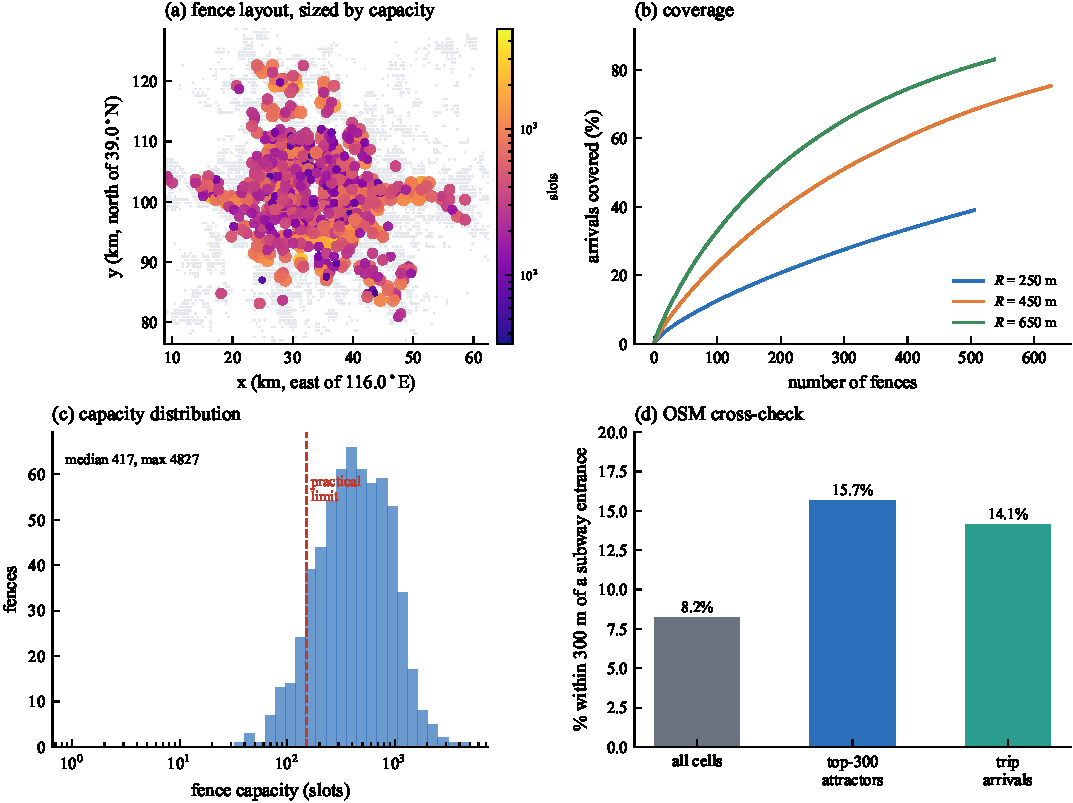
\includegraphics[width=0.9\linewidth]{../figs/fig6_q4.pdf}
\caption[Q4: the 626-fence layout and capacity]{Q4. (a) The 626-fence layout at $R=450$ m, markers sized and coloured by
capacity. (b) Coverage against the number of fences for three walking radii. (c)
Distribution of fence capacity; the dashed line is the 150-slot practical limit. (d)
External check: share of cells, of the top-300 attractors, and of arrivals within
300 m of a subway entrance.}
\label{fig:q4}
\end{figure}


\subsection{How large must each fence be}

The capacities in \figref{fig:q4}c are the most uncomfortable result in this paper.
The median fence needs \textbf{417 slots} and the largest needs \textbf{4{,}827}. At
1.4 m$^2$ per bicycle --- the footprint of a parked bicycle plus its access aisle ---
the plan requires 48.2 hectares of land, the equivalent of 67 football pitches, and the
largest single fence would occupy 0.7 hectares.

The total is not the problem; the distribution is. Every bicycle in the fleet must
stand somewhere, so a 95th-percentile peak, summed over the city, cannot be far from
the fleet: 344{,}463 slots against 343{,}638 bicycles is a 0.2\% margin, and the
agreement is a check on the sizing rather than a coincidence. The
same accounting makes the totals in \tabref{tab:fence} uninformative about layout: the
650 m plan needs 342{,}606 slots and the 450 m plan 344{,}463, within 0.6\% of each
other, because both serve nearly the whole fleet; only the 250 m plan is smaller, and
only because it leaves 61\% of arrivals outside any fence. But
a plan that concentrates 5{,}000 slots on one plaza has not solved parking; it has
formalised the bicycle mountain that electronic fencing was meant to prevent. The
capacity distribution is heavy-tailed because arrivals are: the busiest 10\% of cells
receive 40\% of all trips.

We therefore recommend a \emph{capped} layout rather than an uncapped one. A street
corner can plausibly hold 150 slots --- about 210 m$^2$, a plot ten by twenty-one
metres, the largest a rider can cross in a minute --- and on the uncapped plan
\textbf{89.8\% of fences would exceed it}. Capping instead diverts the excess to the
next fence, and the diversion is exactly the incentive mechanism of
Section~\ref{sec:q3} with the sign reversed: the same reward that fills a deficit cell
can empty an overfull fence, paying the rider to end where there is space.

\subsection{External validation with OpenStreetMap}

The layout is only as good as the demand surface it is built on, and the demand surface
comes from a single operator's data. An independent check is available: if the model's
attractors are real places, they should sit near public transport.

We queried the OpenStreetMap Overpass API for all nodes tagged
\texttt{railway=subway\_entrance} in the study bounding box on 11 November 2026 and
obtained \textbf{1{,}097 entrances} \cite{osm}. The comparison (\figref{fig:q4}d) is
striking. Only 8.2\% of cells lie within 300 m of an entrance, but 15.7\% of the 300
busiest destination cells do --- nearly twice the base rate --- and the median distance
from a top-100 attractor to a subway entrance is \textbf{0.50 km}, against 1.21 km for
a cell chosen at random. Fourteen percent of all arrivals end within 300 m of an
entrance.

The model therefore locates demand where the city's transport infrastructure says it
should be. This does not validate the magnitudes --- an external source cannot do that
--- but it validates the geography, which is what the fence layout depends on.

